\beginsong{Es ist an der Zeit}[wuw={Eric Bogle, 1976 (freie deutsche Nachdichtung durch Hannes Wader, 1980)}, pfii={86}, pfiii={43}, index={Weit in der Champagne}]

\markboth{\songtitle}{\songtitle}

\beginverse
\endverse
\centering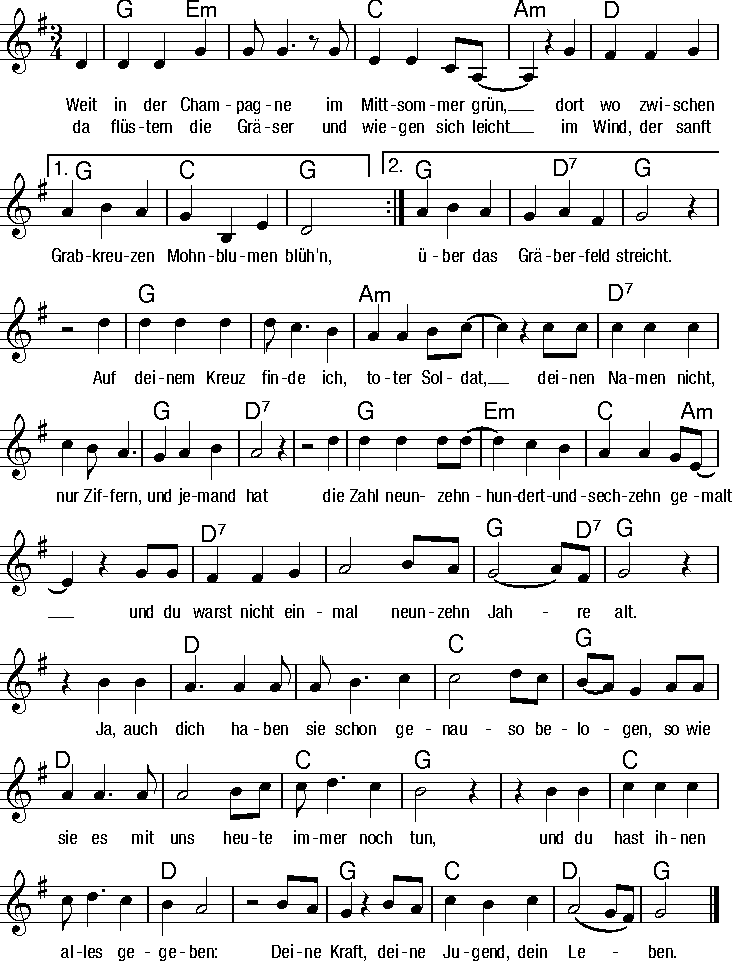
\includegraphics[width=1\textwidth]{Noten/Lied036.pdf}	

%\centering\includegraphics[width=1\textwidth]{Noten/Lied036_1.pdf}	


\beginverse\memorize
\[G]Hast du, toter Sol\[Em]dat, mal ein \[C]Mädchen ge\[Am]liebt?
Sicher \[D]nicht, denn nur dort, wo es \[G]Frie\[C]den \[G]gibt,
\[G]können Zärtlichkeit \[Em]und Ver\[C]trauen ge\[Am]deih'n.
Warst \[D]Soldat, um zu sterben, nicht \[G]um jung \[D]zu \[G]sein.
Viel\[G]leicht dachtest \[Em]du dir: Ich \[Am]falle schon bald,
nehme \[D7]mir mein Vergnügen, wie es \[G]kommt, mit Ge\[D7]walt.
Dazu \[G]warst du ent\[Em]schlossen, hast \[Am]dich aber dann
vor \[D]dir selber geschämt und es doch \[G]nie \[D]ge\[G]tan.
\endverse

\beginchorus
Ja, auch \[D]dich haben sie schon \[C]genauso \[G]belogen,
so, wie \[D]sie es mit uns heute \[C]immer noch \[G]tun,
und du \[C]hast ihnen alles \[D]gegeben:
Deine \[G]Kraft, deine \[C]Jugend, dein \[D]Le\[G]ben.
\endchorus

\beginverse
^Soldat, gingst du ^gläubig und ^gern in den ^Tod?
Oder ^hast du verzweifelt, ver^bittert, ^ver^roht
^deinen wirklichen ^Feind nicht er^kannt bis zum ^Schluss?
^Ich hoffe, es traf dich ein sau^be^rer ^Schuss.
Oder ^hat ein Ge^schoss dir die ^Glieder zerfetzt?
Hast du ^nach deiner Mutter ge^schrien bis zu^letzt?
Bist du ^auf deinen ^Beinstümpfen ^weitergerannt?
Und ^dein Grab, ^birgt es mehr als ein Bein, ^eine ^Hand?
\endverse
%\renewcommand{\everychorus}{\textnote{\bf Refrain (wdh.)}}

\beginchorus
Ja, auch \[D]dich haben sie schon \[C]genauso \[G]belogen,
so, wie \[D]sie es mit uns heute \[C]immer noch \[G]tun,
und du \[C]hast ihnen alles \[D]gegeben:
Deine \[G]Kraft, deine \[C]Jugend, dein \[D]Le\[G]ben.
\endchorus

\beginverse
^Es blieb nur das ^Kreuz als ^einzige ^Spur
von ^deinem Leben, doch ^hör' mei^nen ^Schwur
^für den Frieden zu ^kämpfen und ^wachsam zu ^sein.
^Fällt die Menschheit noch einmal auf Lü^gen ^he^rein,
dann ^kann es ge^scheh'n, dass bald ^niemand mehr lebt,
niemand, ^der die Milliarden von ^Toten be^gräbt.
Doch längst ^finden sich ^mehr und mehr ^Menschen bereit,
die^sen Krieg zu verhindern, es ist ^an ^der ^Zeit.
\endverse

\beginchorus
Ja, auch \[D]dich haben sie schon \[C]genauso \[G]belogen,
so, wie \[D]sie es mit uns heute \[C]immer noch \[G]tun,
und du \[C]hast ihnen alles \[D]gegeben:
Deine \[G]Kraft, deine \[C]Jugend, dein \[D]Le\[G]ben.
\endchorus

\endsong

\beginscripture{}
Das Lied ist die deutsche Variante von ''The green fields of France'' von Eric Bogle und wurde in dieser Version zu einer Hymne der Friedensbewegung in den 1980er Jahren.
\endscripture

\begin{intersong}

\end{intersong}